\documentclass[french, a4paper, 12pt, openany]{book}
\usepackage{graphicx}
\usepackage[utf8]{inputenc}
\usepackage[T1]{fontenc}
\usepackage{babel}
\usepackage{amssymb}
\usepackage{amsmath}
\usepackage[top=2cm, bottom=2cm, left=2cm, right=2cm]{geometry}

\title{\Huge{Rapport Travaux Pratiques \\ SC3}}
\author{\\ Théo Bertrand \& Xyléan Broeders \\ Fi 2021}
\date{19 Décembre 2018}

\begin{document}

%Title of the document
\maketitle

\chapter{Analyse du signal}
	Durant ce TP, nous allons nous intéresser à l'étude d'un signal (ici le n\textsuperscript{o}8). Dans un premier temps, nous allons étudier les caractéristiques physiques du signal.  Pour ensuite, pouvoir déterminer si ce signal est stationnaire du second ordre. Finalement, nous allons essayer (dans la mesure du possible) de reconstituer le signal d'origine.
\section{Etude générale du signal}
	Nous observons tout d'abord que les valeurs de ce signal à une amplitude de 6 volts, et une durée de 500 $\mu s$ (1 $\mu s$ par fenetre d'échantillonnage). Intéressons-nous maintenant à plusieurs de ses caractéristiques et notamment sa moyenne, sa variance, et son autocorrélation.
  \begin{figure}[ht]
    \begin{center}
    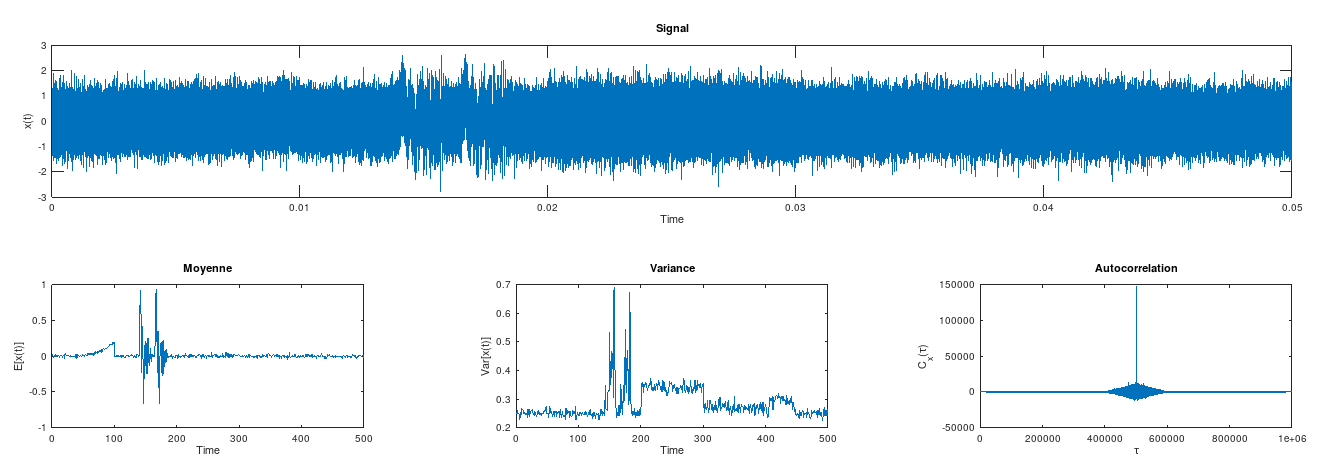
\includegraphics[scale=0.25]{images/SignalFull.png}
    \end{center}
    \caption{Recapitulatif des valeurs obtenues}
    \label{Recapitulatif des valeurs obtenues}
  \end{figure}

\section{Stationnarité du 2\textsuperscript{nd} orde}
	Pour rappel, un signal est dit stationnaire du second ordre si ses propriétés statistiques ne varient pas en fonctions du temps. C'est-à-dire s'il vérifie :
  \begin{center}
  	\begin{math}\mathbb{E}[X(t)^2]<\infty\end{math} \\
  	\begin{math}\mathbb{E}[X(t)]=Constante\end{math} \\
  	\begin{math}\mathbb{E}[X(t)X(t)^*(t-\tau)]=C_X(\tau)\end{math}
  \end{center}
	\newpage

	\begin{figure}[ht]
		\begin{center}
		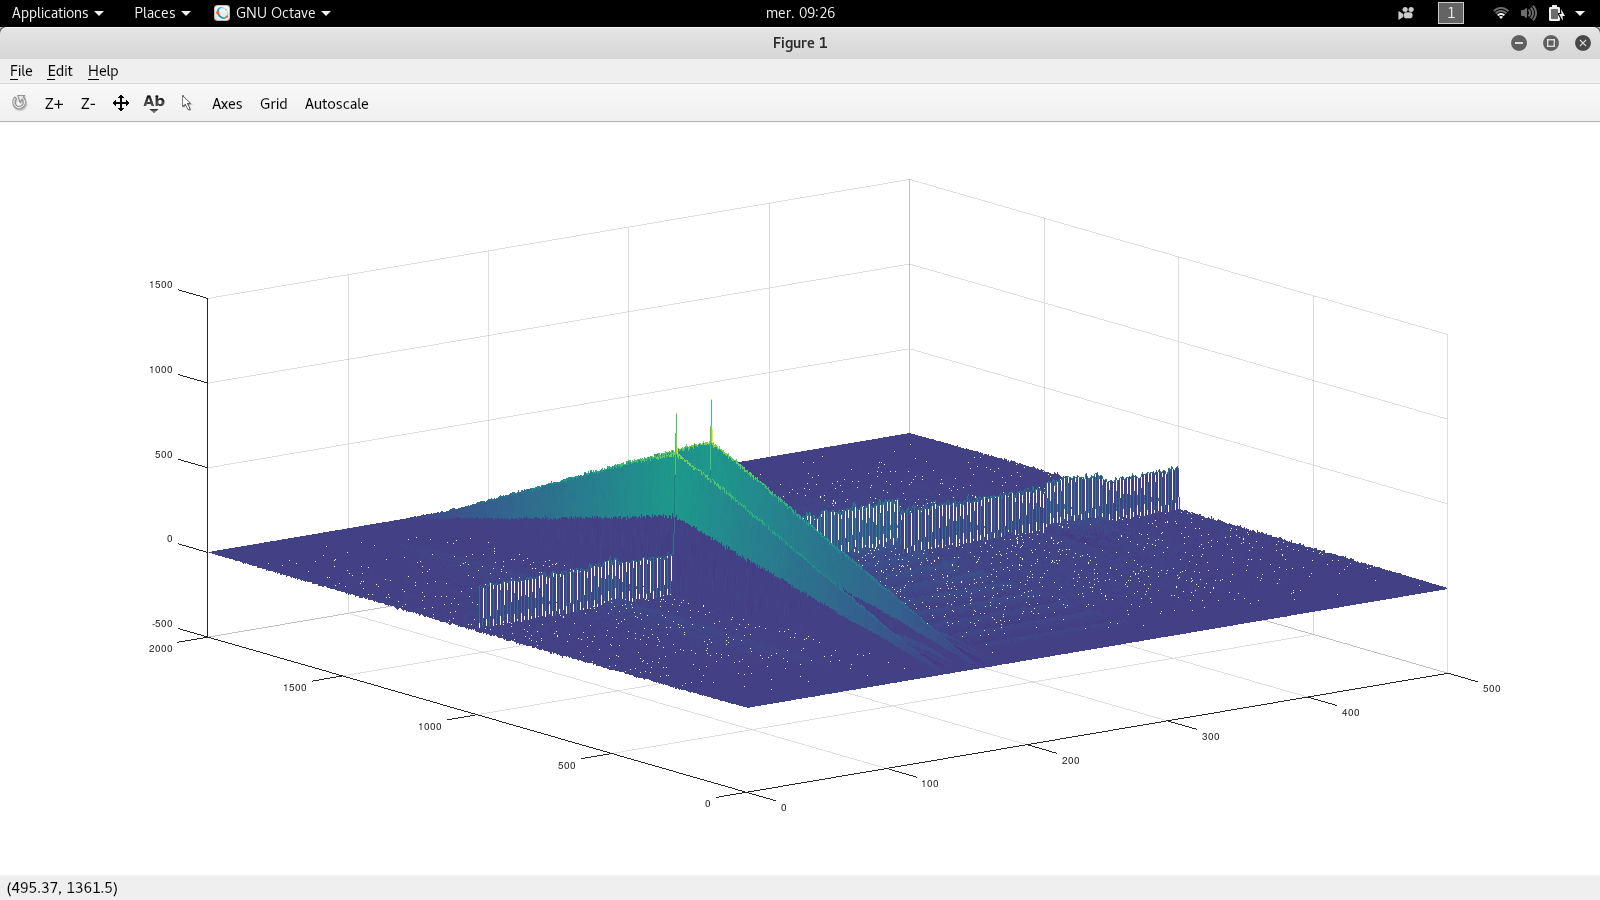
\includegraphics[scale=0.25]{images/AutoCorrFull.png}
		\end{center}
		\caption{Recapitulatif des valeurs obtenues}
		\label{Recapitulatif des valeurs obtenues}
	\end{figure}

	Après étude de l'autocorrélation, on constate que le signal n'est pas stationnaire du second ordre, en effet son autocorrélation dépendant du temps. Néanmoins, nous observons qu'elle est constante sur certains intervalles de temps. On peut ainsi dénombrer 4 "blocs" :

  \begin{description}
    \item[Bloc 1 : ]de 0 à 100 000
    \item[Bloc 2 : ]de 100 000 à 136 000
    \item[Bloc 3 : ]de 136 000 à 190 000
    \item[Bloc 4 : ]de 190 000 à 500 000
  \end{description}
  \subsection{Bloc 1}
	\begin{figure}[ht]
    \begin{center}
    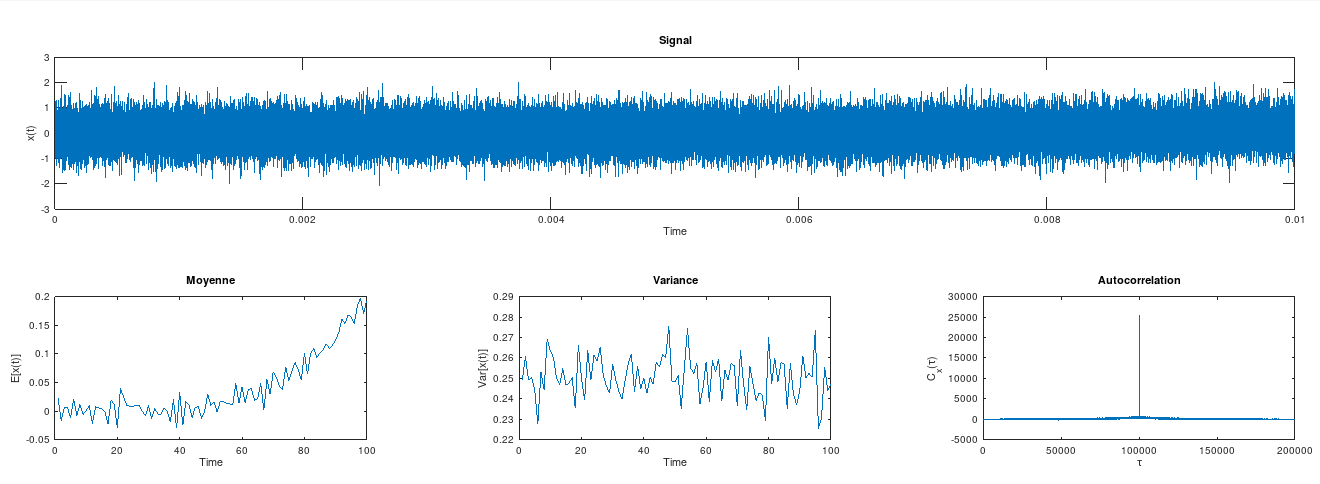
\includegraphics[scale=0.25]{images/SignalBloc1.png}
    \end{center}
    \caption{Analyses du Bloc 1}
    \label{Analyses du Bloc 1}
  \end{figure}

	\begin{figure}[ht]
		\begin{center}
		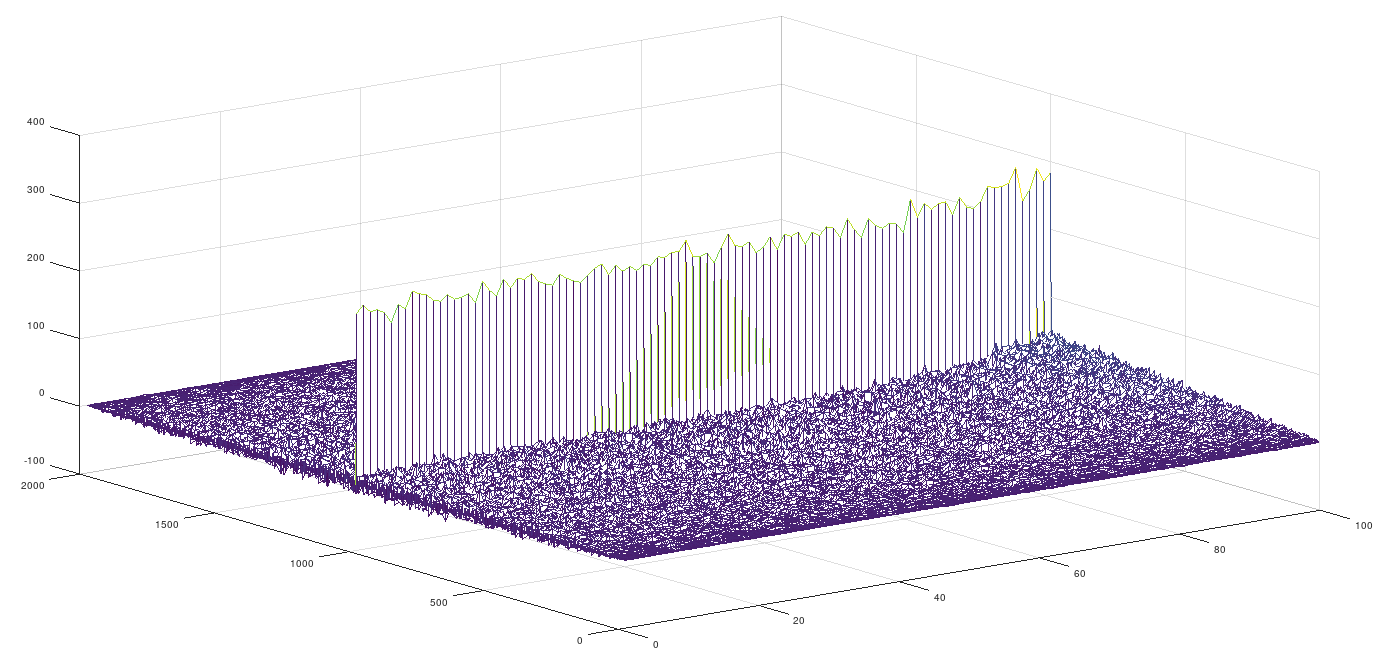
\includegraphics[scale=0.25]{images/AutoCorrBloc1.png}
		\end{center}
		\caption{Analyses de l'autocorrelation Bloc 1}
		\label{Analyses de l'autocorrelation Bloc 1}
	\end{figure}

	L'éspérence et l'autocorrelation étant dépendantes du temps, ce signal n'est pas stationnaire du second ordre.
  \subsection{Bloc 2}

	\begin{figure}[ht]
		\begin{center}
		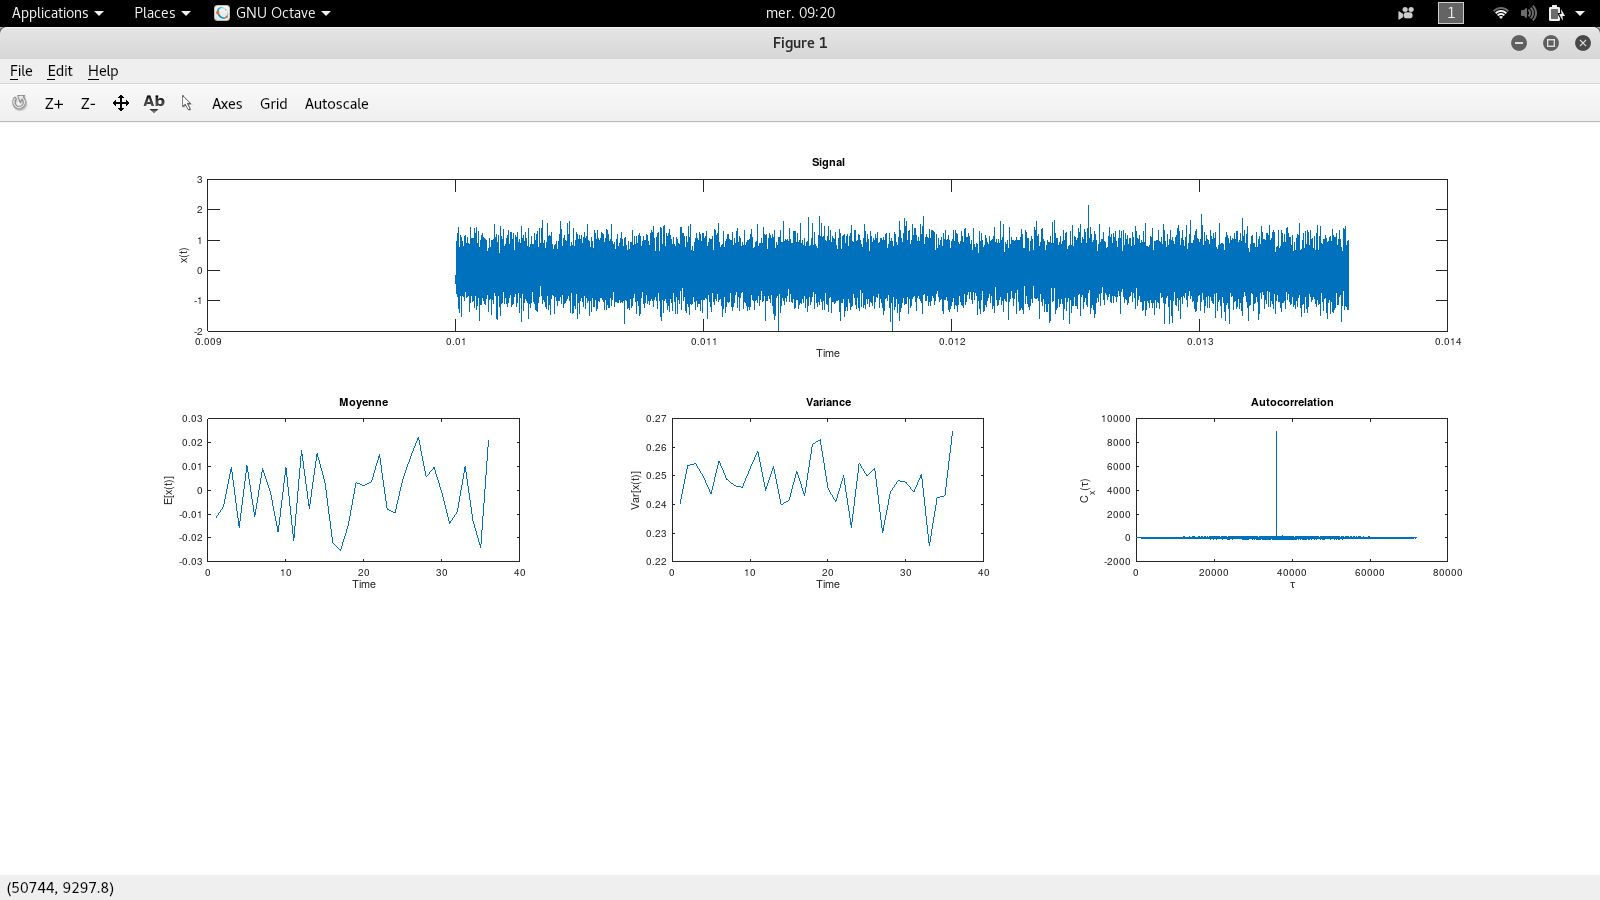
\includegraphics[scale=0.25]{images/SignalBloc2.png}
		\end{center}
		\caption{Analyses du Bloc 2}
		\label{Analyses du Bloc 2}
	\end{figure}

	\begin{figure}[ht]
		\begin{center}
		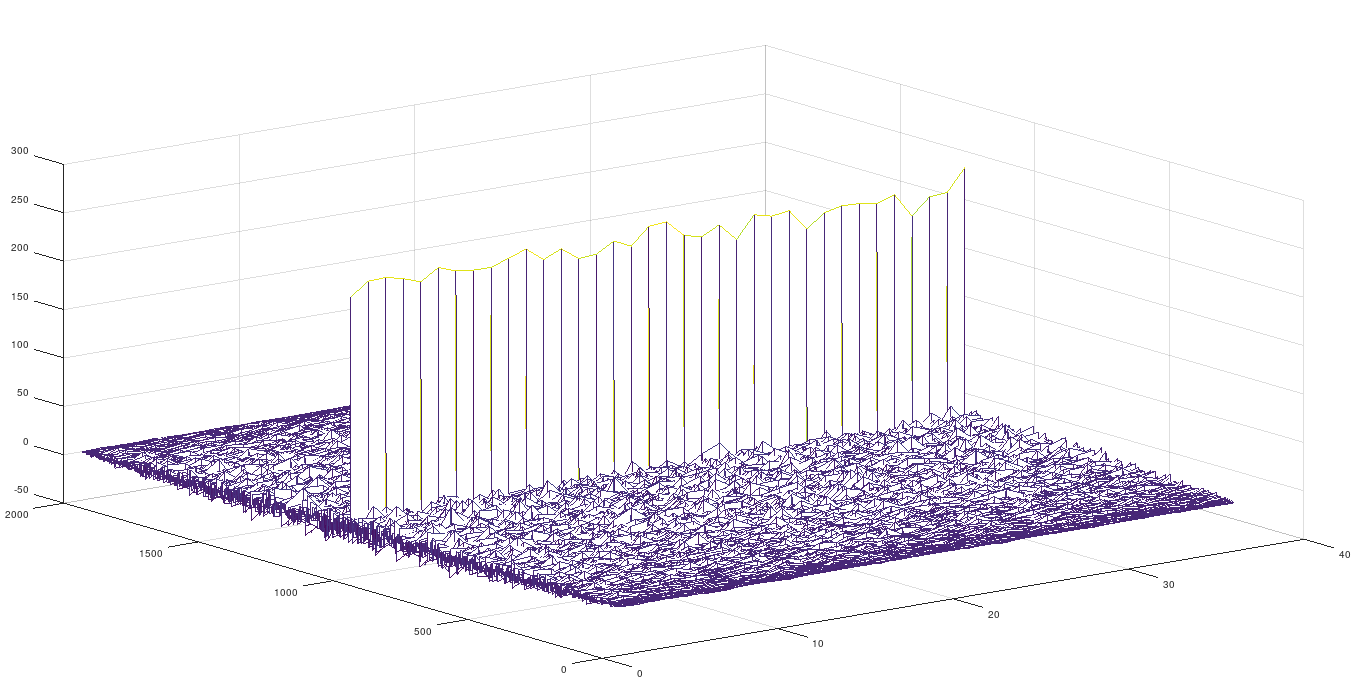
\includegraphics[scale=0.25]{images/AutoCorrBloc2.png}
		\end{center}
		\caption{Analyses de l'autocorrelation Bloc 2}
		\label{Analyses de l'autocorrelation Bloc 2}
	\end{figure}

	Les variations de l'éspérance peuvent être considérées comme négligeables (amplitude de 0,4 volt). De même son autocorrélation peut être comme constante.
	Après étude de la variance et sachant que \begin{math}Var(X) = \mathbb{E}[X(t)^2] - \mathbb{E}[X(t)]^2\end{math}, et que \begin{math}\mathbb{E}[X(t)]^2<\infty\end{math}, car l'éspérance est constante, alors on a bien : \begin{math}\mathbb{E}[X(t)^2]<\infty\end{math}. Ce bloc est donc bien stationnaire du second ordre.
	Enfin, on constate un pic de Dirac en \(t = 0\), ce qui est la preuve de la précense de bruit dans le signal.

	\begin{figure}[ht]
		\begin{center}
		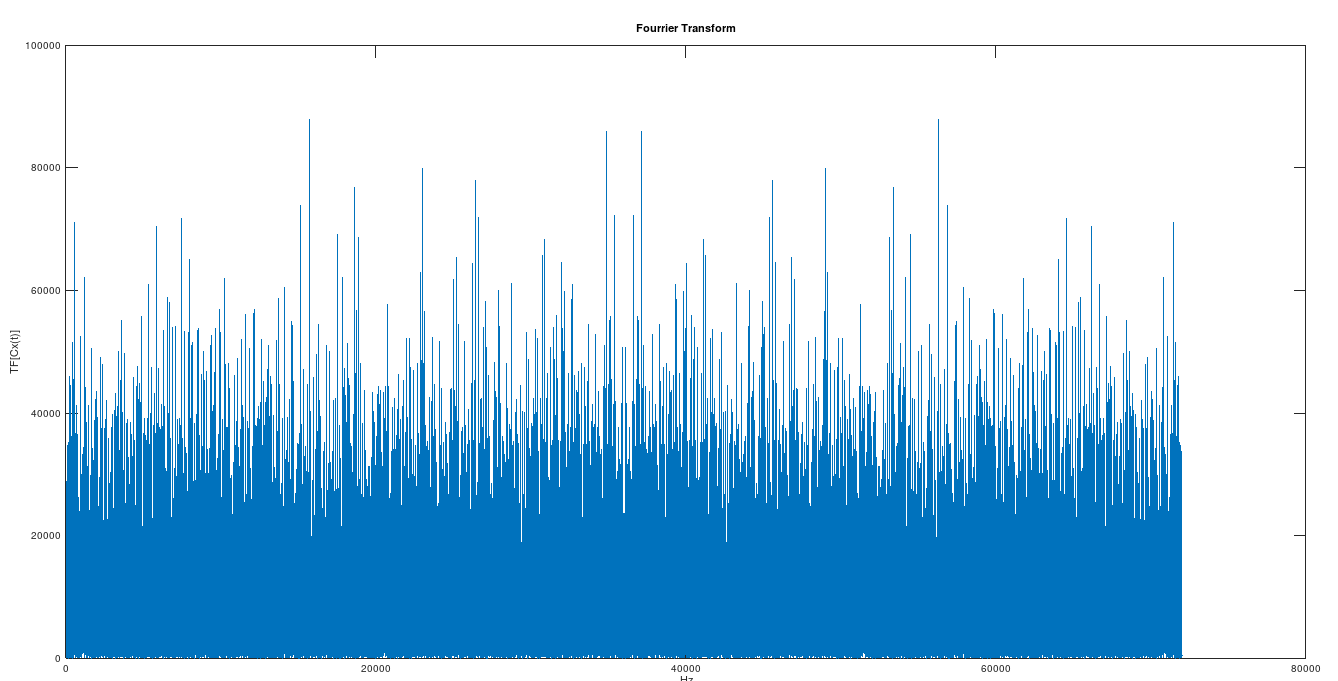
\includegraphics[scale=0.25]{images/DSPBloc2.png}
		\end{center}
		\caption{Analyses de la DSP du Bloc 2}
		\label{Analyses de la DSP du Bloc 2}
	\end{figure}

	Après analyse de la Densité Spéctrale de Puissance, on la suppose constante. \\
	Sachant que, par definition un bruit blanc est stationnaire du second ordre, à une éspérance nulle et à une DSP constante. On en déduit donc que le Bloc 2 est un bruit blanc. Cela ce confirme lors de l'étude de la \textit{Fast Fourier Transform} du Bloc 2.

	\begin{figure}[ht]
		\begin{center}
		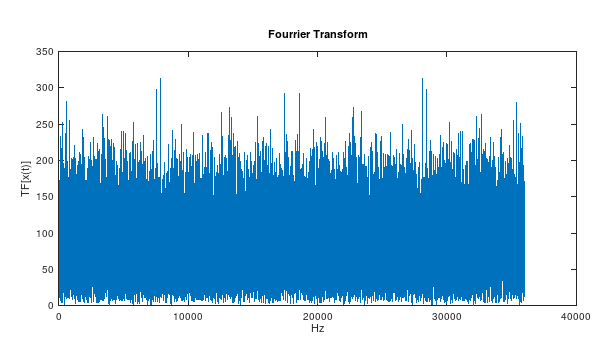
\includegraphics[scale=0.25]{images/TFBloc2.png}
		\end{center}
		\caption{Fast Fourier Transform du Bloc 2}
		\label{Fast Fourier Transform du Bloc 2}
	\end{figure}

  \subsection{Bloc 3}

	\begin{figure}[ht]
		\begin{center}
		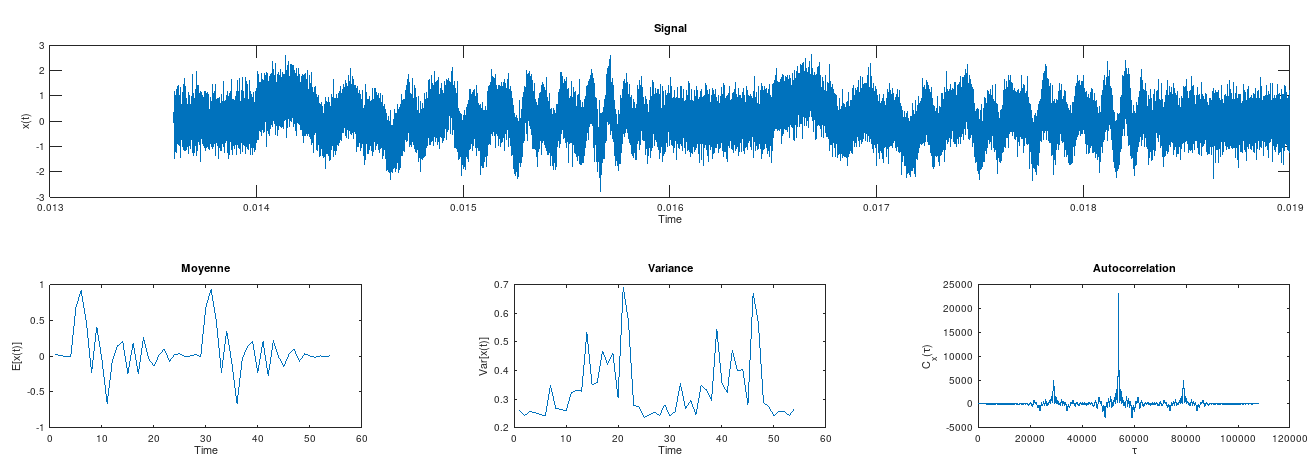
\includegraphics[scale=0.25]{images/SignalBloc3.png}
		\end{center}
		\caption{Analyses du Bloc 3}
		\label{Analyses du Bloc 3}
	\end{figure}

	\begin{figure}[ht]
		\begin{center}
		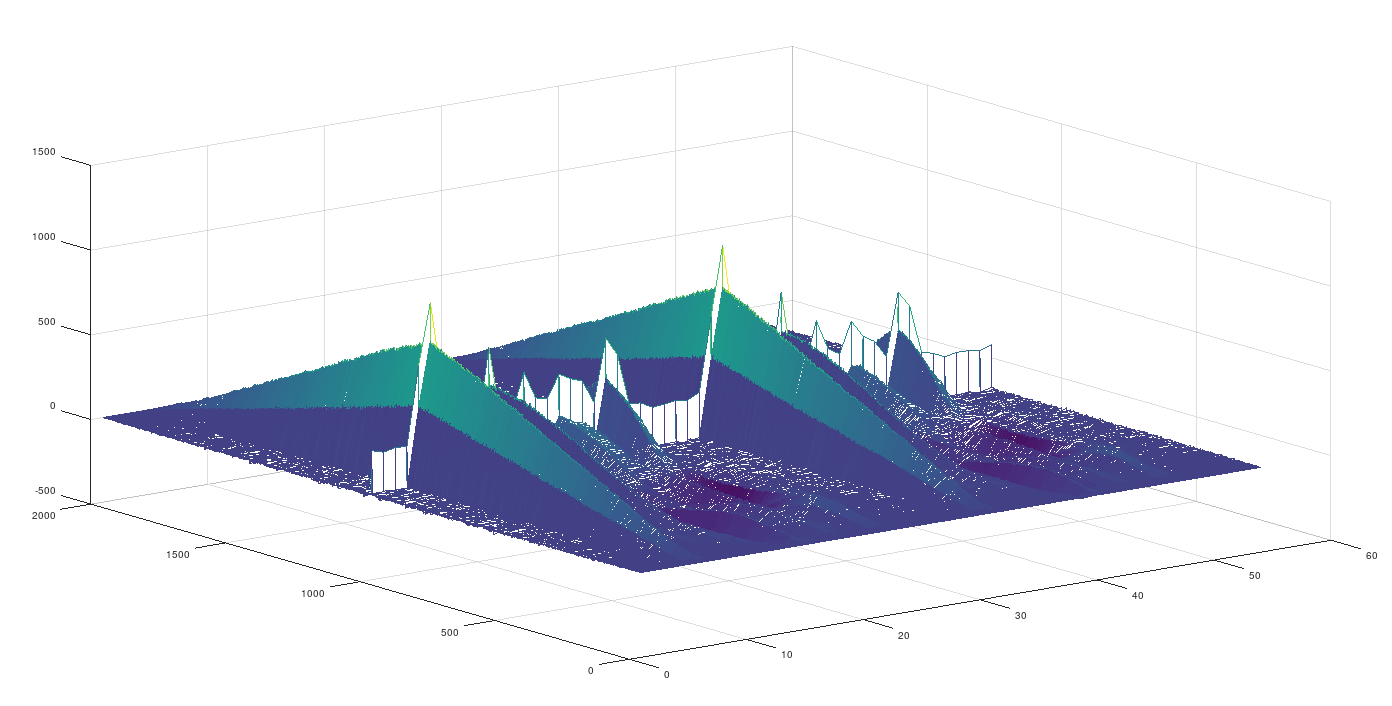
\includegraphics[scale=0.25]{images/AutoCorrBloc3.png}
		\end{center}
		\caption{Analyses de l'autocorrelation Bloc 3}
		\label{Analyses de l'autocorrelation Bloc 3}
	\end{figure}

	L'éspérence et l'autocorrelation étant dépendantes du temps, ce signal n'est pas stationnaire du second ordre.
  \subsection{Bloc 4}

	\begin{figure}[ht]
    \begin{center}
    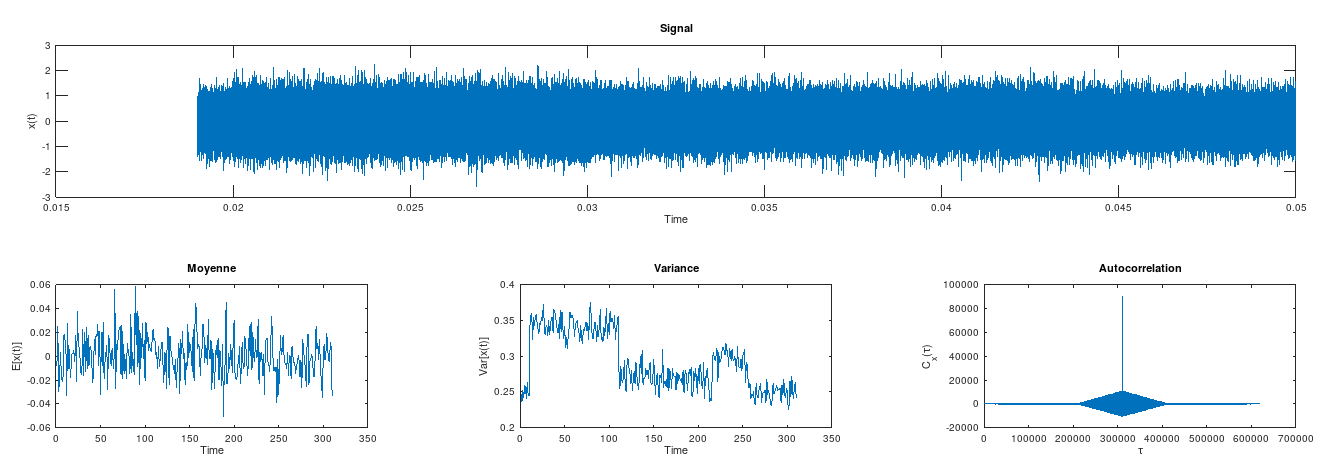
\includegraphics[scale=0.25]{images/SignalBloc4.png}
    \end{center}
    \caption{Analyses du Bloc 4}
    \label{Analyses du Bloc 4}
  \end{figure}

	\begin{figure}[ht]
		\begin{center}
		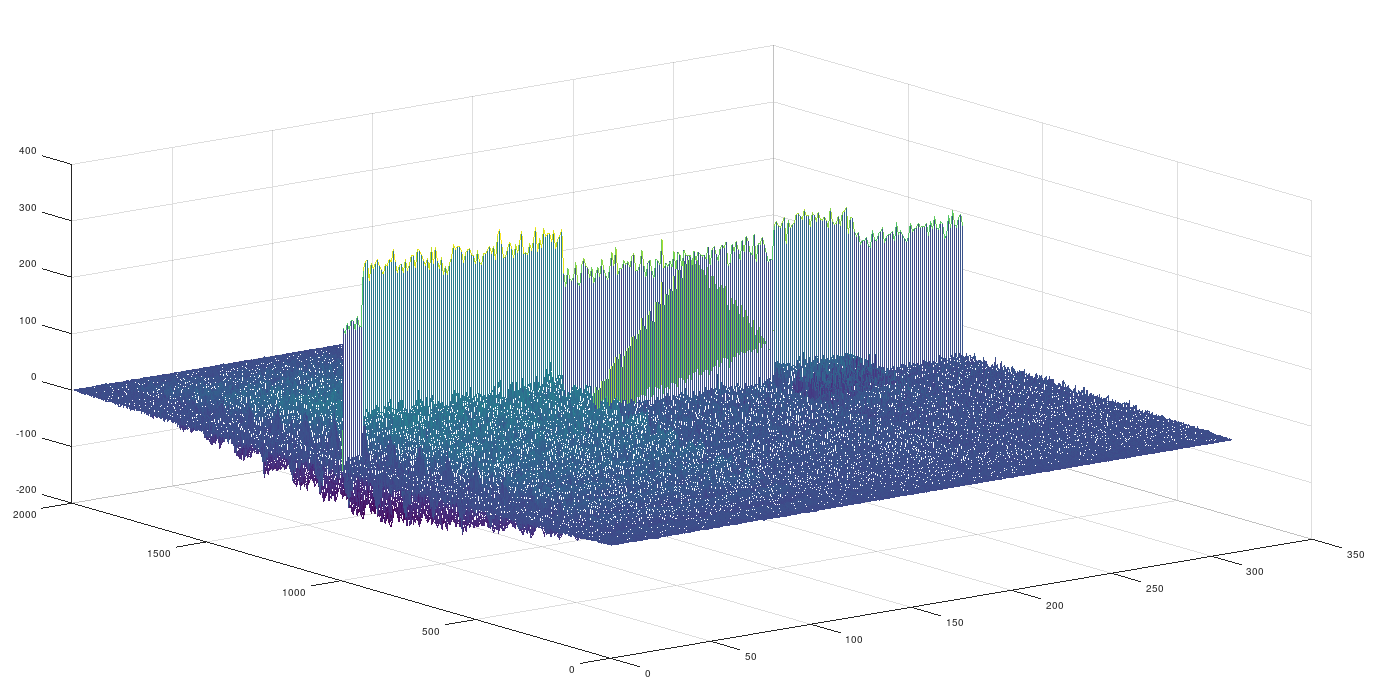
\includegraphics[scale=0.25]{images/AutoCorrBloc4.png}
		\end{center}
		\caption{Analyses de l'autocorrelation Bloc 4}
		\label{Analyses de l'autocorrelation Bloc 4}
	\end{figure}

	Lors de l'étude l'autocorrelation de ce bloc, nous avons constater la précense de deux sous-blocs, noté Bloc 4a (190 000 - 300 000) et Bloc 4b (300 000 - 500 000). En effet, l'un à une autocorrelation variant dans le temps (Bloc 4a), contrairement à l'autre (Bloc 4b).

	\subsubsection{Bloc 4a}
	L'éspérence étant dépendantes du temps, ce signal n'est pas stationnaire du second ordre.

	\subsubsection{Bloc 4b}

	\begin{figure}[ht]
		\begin{center}
		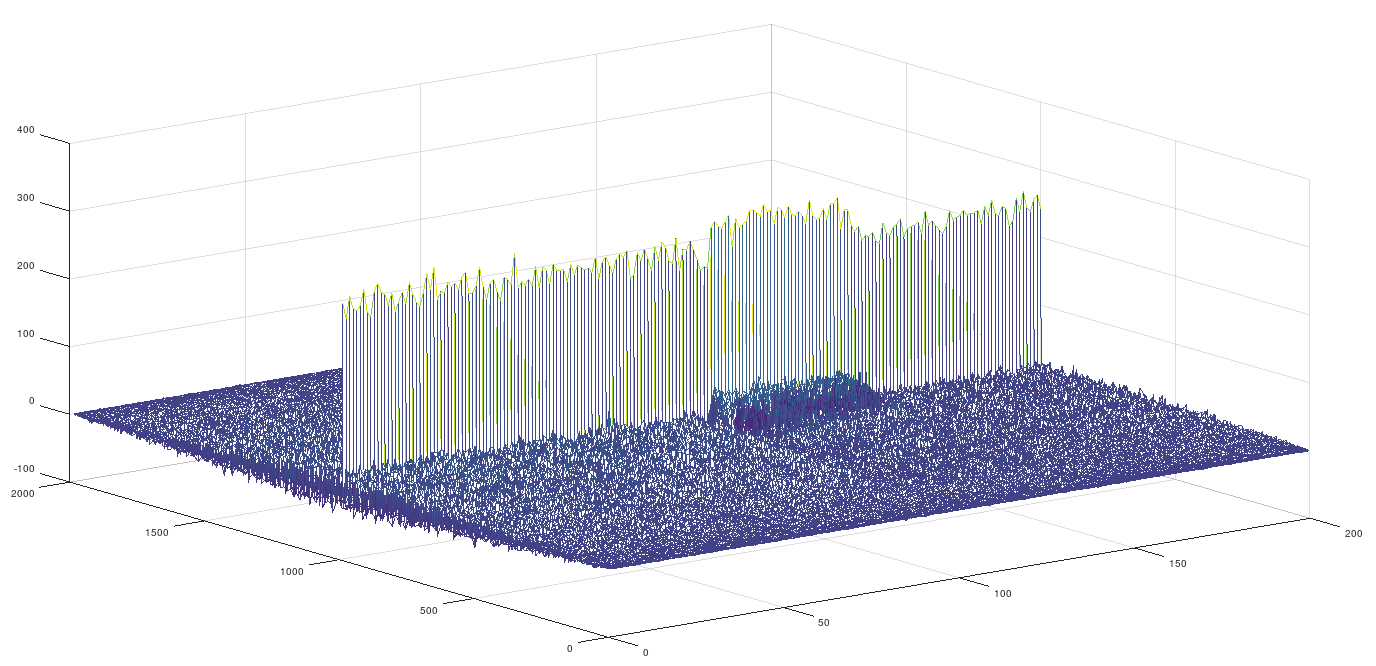
\includegraphics[scale=0.25]{images/AutoCorrBloc4-2.png}
		\end{center}
		\caption{Analyses de l'autocorrelation Bloc 4b}
		\label{Analyses de l'autocorrelation Bloc 4b}
	\end{figure}

	Les variations de l'éspérance peuvent être considérées comme négligeables. De même son autocorrélation peut être comme constante.
	Après étude de la variance et sachant que \begin{math}Var(X) = \mathbb{E}[X(t)^2] - \mathbb{E}[X(t)]^2\end{math}, et que \begin{math}\mathbb{E}[X(t)]^2<\infty\end{math}, car l'éspérance est constante, alors on a bien : \begin{math}\mathbb{E}[X(t)^2]<\infty\end{math}. Ce bloc est donc bien stationnaire du second ordre.
	Enfin, on constate un pic de Dirac en \(t = 0\), ce qui est la preuve de la précense de bruit dans le signal.

	\begin{figure}[ht]
		\begin{center}
		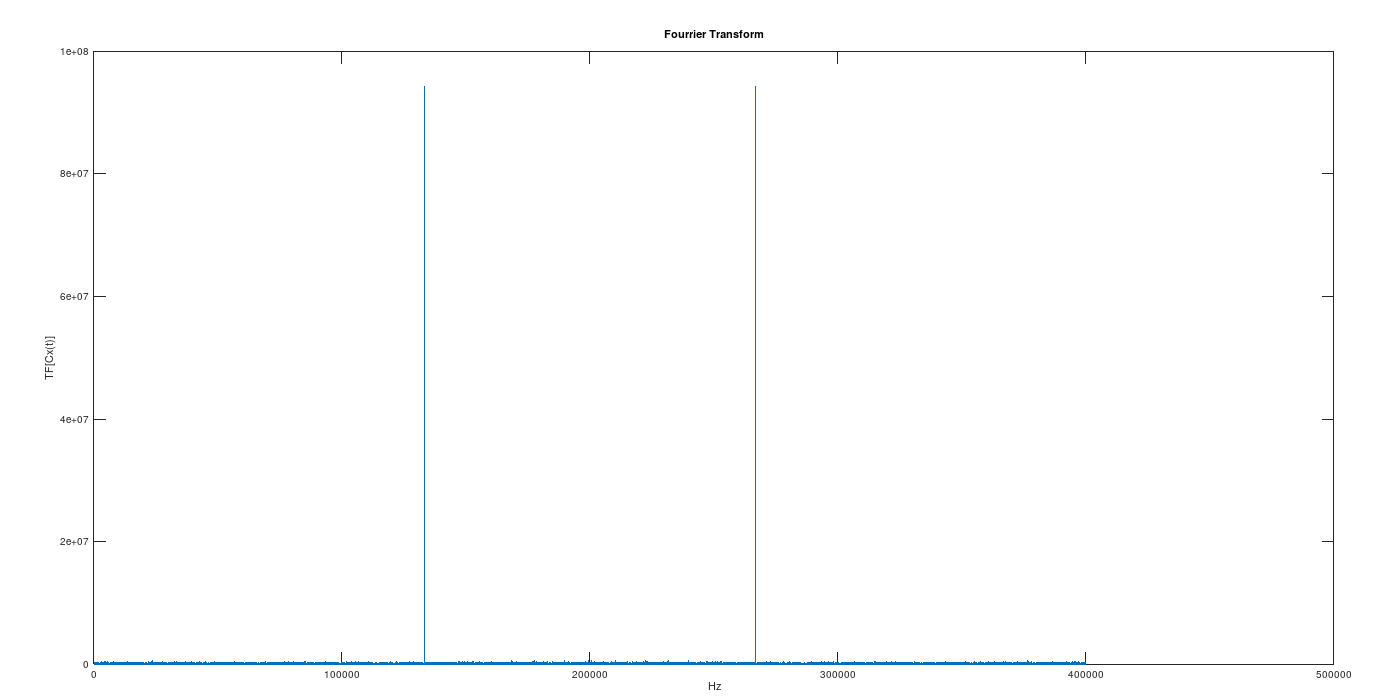
\includegraphics[scale=0.25]{images/DSPBloc4-2.png}
		\end{center}
		\caption{Analyses de la DSP du Bloc 4b}
		\label{Analyses de la DSP du Bloc 4b}
	\end{figure}

	\begin{figure}[ht]
		\begin{center}
		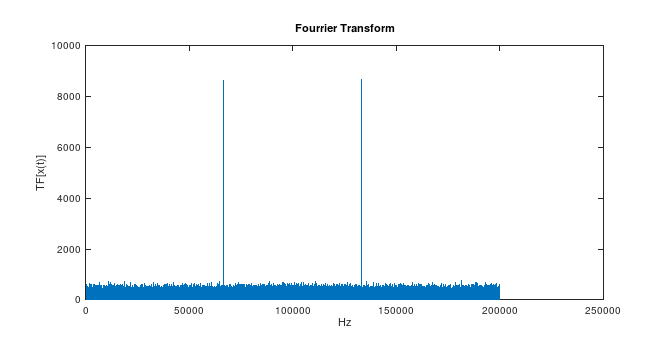
\includegraphics[scale=0.5]{images/TFBloc4-2.png}
		\end{center}
		\caption{Fast Fourier Transform du Bloc 4b}
		\label{Fast Fourier Transform du Bloc 4b}
	\end{figure}

	Après analyse de la Densité Spéctrale de Puissance, on la suppose constante. \\
	Après étude de la \textit{Fast Fourier Transform} du Bloc 4b, constate deux pics de Dirac en \begin{math}-f_0 \end{math} et \begin{math}f_0\end{math}. Sachant que :
	\begin{center}
		\begin{math}TF[cos(X)] = \frac{1}{2}[\delta (f - f_0) + \delta (f + f_0)]\end{math}
	\end{center}
	On en déduit donc la précense d'une fonction cosinus dans ce bloc.


\chapter{Lancement des fonctions}
\end{document}
